\subsection{Konstante globale Problemmenge}
In einem ersten Schritt wurde versucht alle Probleme mithilfe einer konstanten, globalen Problemmenge zu lösen. Dabei fiel auf, dass dieser Algorithmus, unabhängig vom Problem, mit sowohl der Grösse der Problemmenge als auch der Anzahl Lösungskandidaten skaliert. Sehr gut sieht man dies an Abbildung \ref{fig:c_g_div5}. Auf der X-Achse sind sowohl die Grösse der Problemmenge (z.B. $P:50$) als auch die Anzahl Lösungskandidaten (z.B. $C:100$) abgebildet. Auf der Y-Achse sieht man die Performance des Algorithmus bei den jeweiligen Eingabeparametern.

\begin{figure}[h]
  \centering
  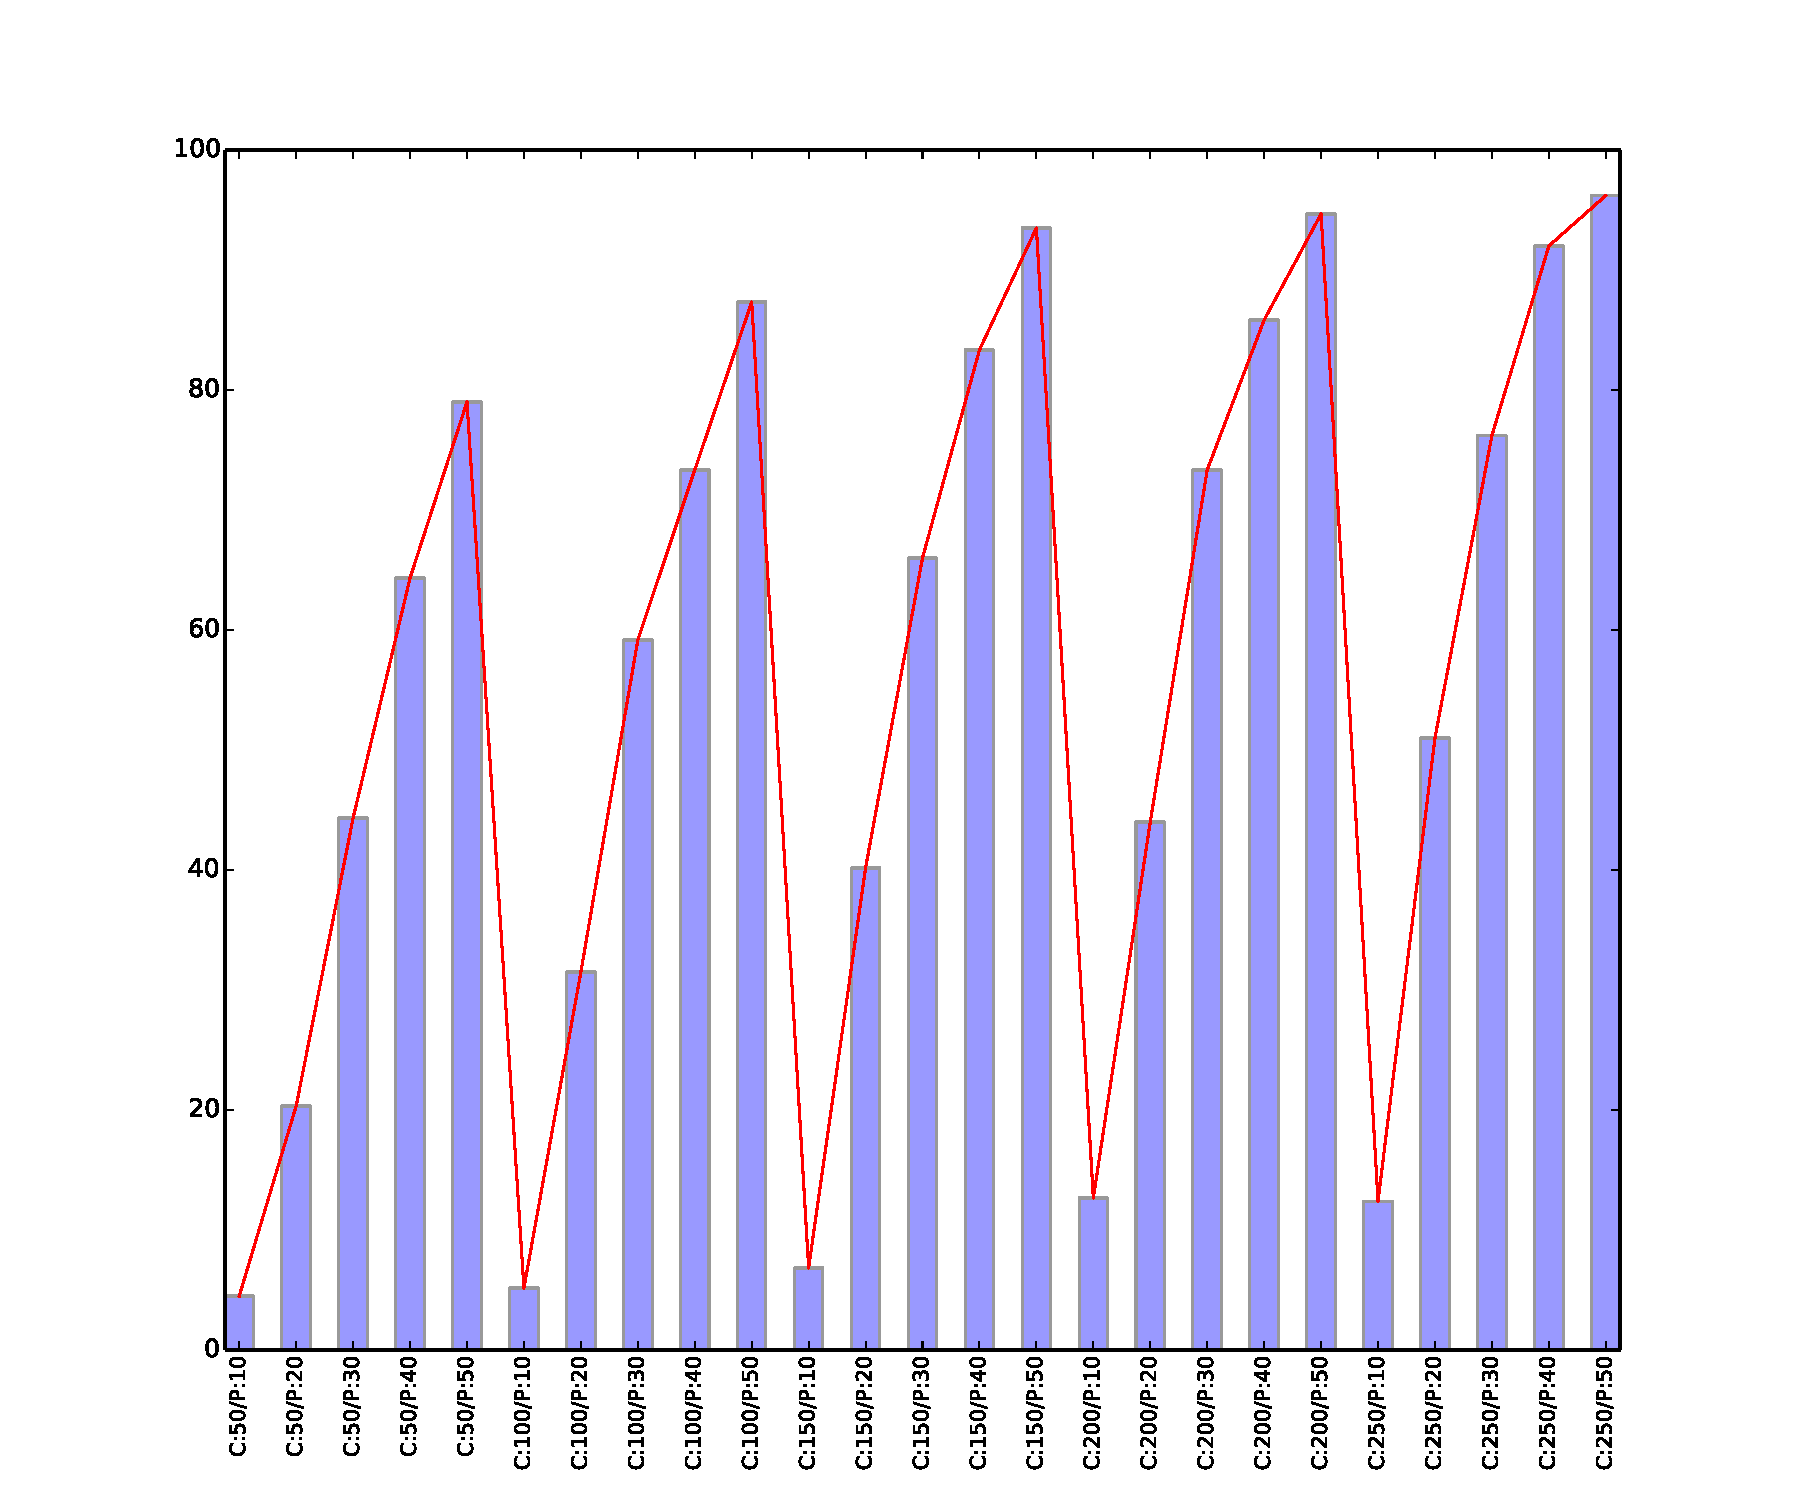
\includegraphics[width=0.8\textwidth]{images/C_G_div5_solved.pdf}
  \caption[Durch fünf teilbar Problem - KG Algorithmus]{Durch fünf teilbar Problem - KG Algorithmus}
  \label{fig:c_g_div5}
\end{figure}

Die Eingabeparameter für die Abbildung \ref{fig:c_g_div5} waren:
\begin{itemize}
	\item Grösse der Problemmenge: 10, 20, 30, 40, 50
	\item Anzahl der Lösungskandidaten: 50, 100, 150, 250
\end{itemize}

In dieser Abbildung zeichnet sich ein \flqq haifischzahnförmiges\frqq Muster ab, was darauf schliessen lässt, dass dieser Algorithmus mit zu kleinen Problemmengen sehr schlecht konvergiert. Dies kann auch nur teilweise durch die Verwendung von mehr Lösungskandidaten wettgemacht werden. Um dies weiter zu untersuchen wurden bei dieser Aufgabenstellung (durch fünf Teilbar) Tests bei konstanter Anzahl Lösugskandidaten durchgeführt. 

\begin{figure}[h]
  \centering
  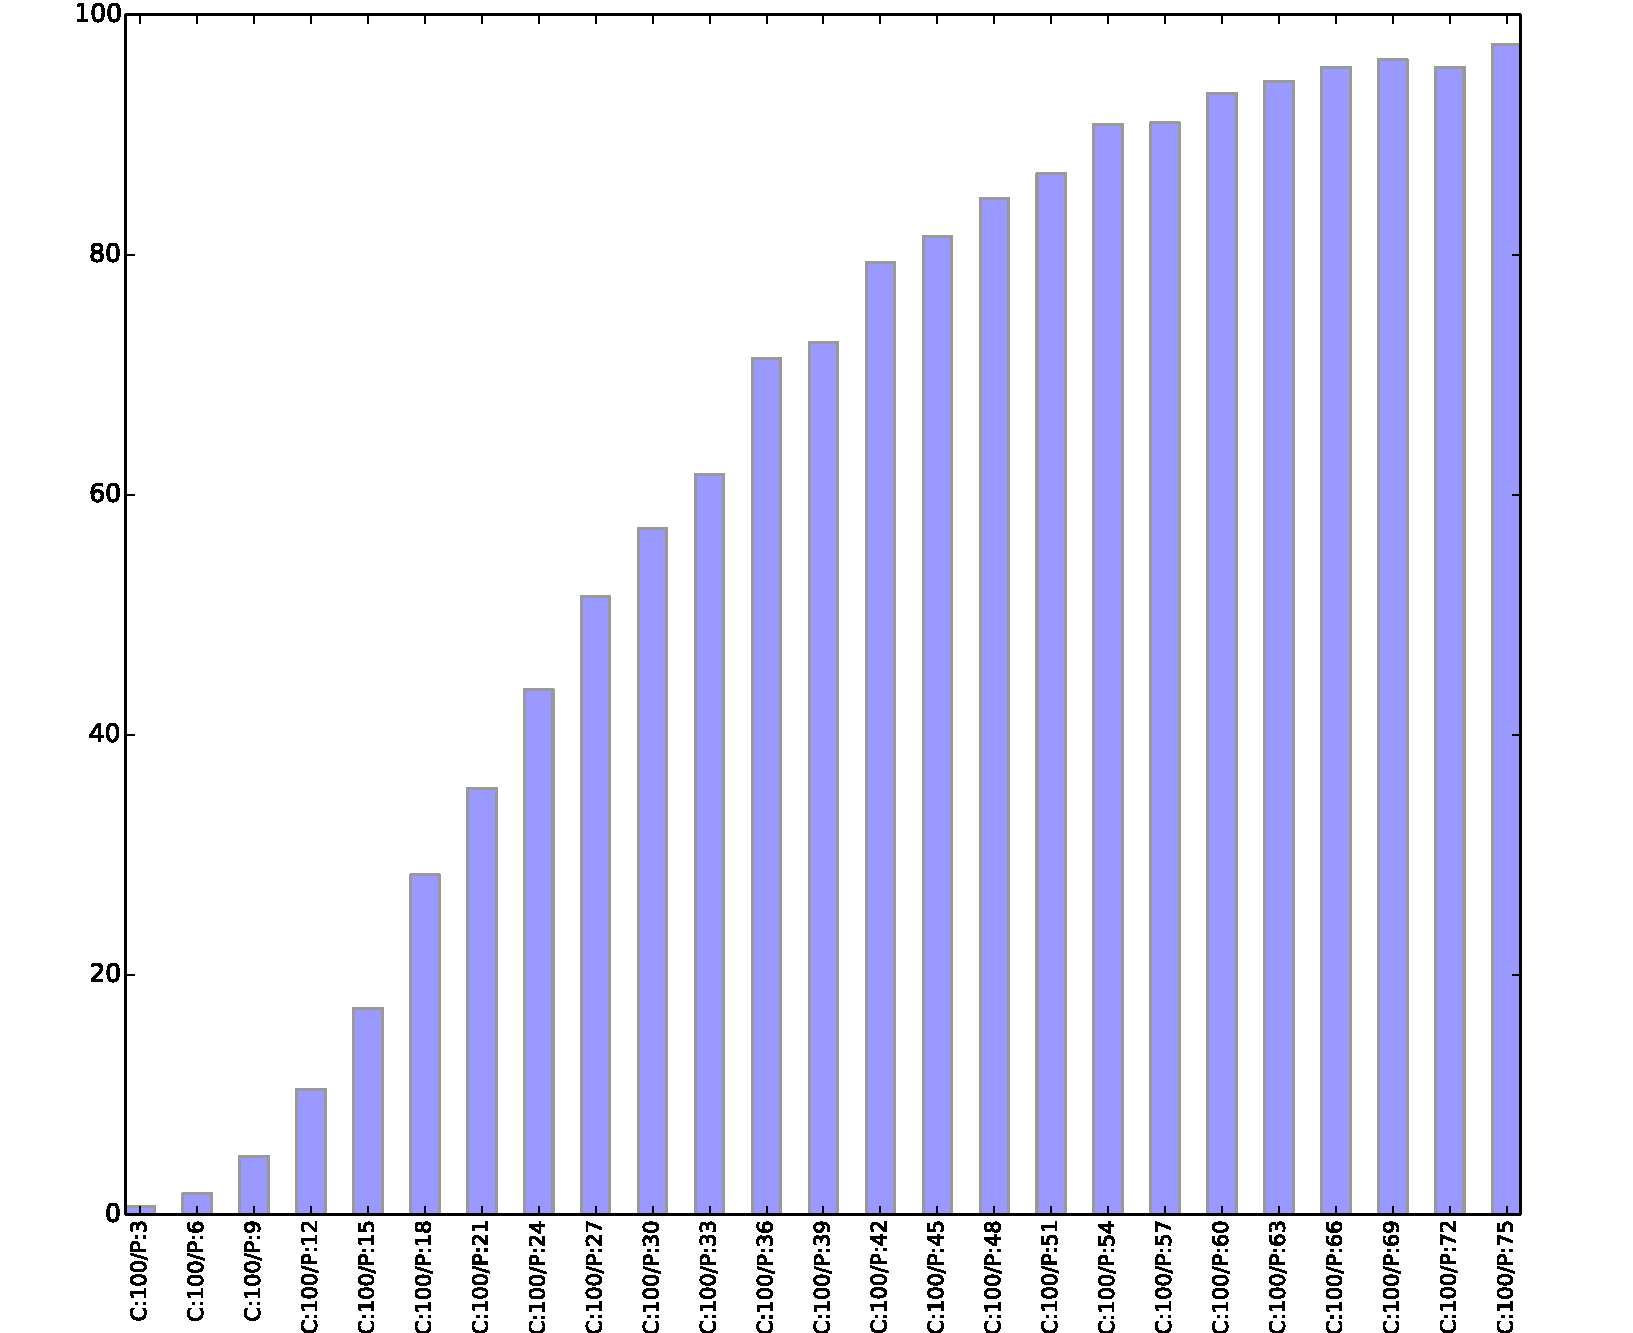
\includegraphics[width=0.78\textwidth]{images/C_G_PS_div5PS_solved.pdf}
  \caption[KG Algorithmus - Skalierung mit Problemmengengrösse]{KG Algorithmus - Skalierung mit Problemmengengrösse}
  \label{fig:c_g_ps_div5}
\end{figure}

Die Eingabeparameter für die Abbildung \ref{fig:c_g_ps_div5} waren:
\begin{itemize}
	\item Grösse der Problemmenge: 3, 6, 9, 12, ..., 72, 75
	\item Anzahl der Lösungskandidaten: 100
\end{itemize}

In Abbildung \ref{fig:c_g_ps_div5} sieht man wie eine zu kleine Problemmenge den Erfolg des Algorithmus einschränken kann. Jedoch flacht die Kurve ab circa 40 Problemen langsam ab und ab circa 65 Problemen scheint eine Vergrösserung der Problemmenge zu keiner signifikanten Verbesserung des Ergebnisses mehr zu führen.

\begin{figure}[H]
  \centering
  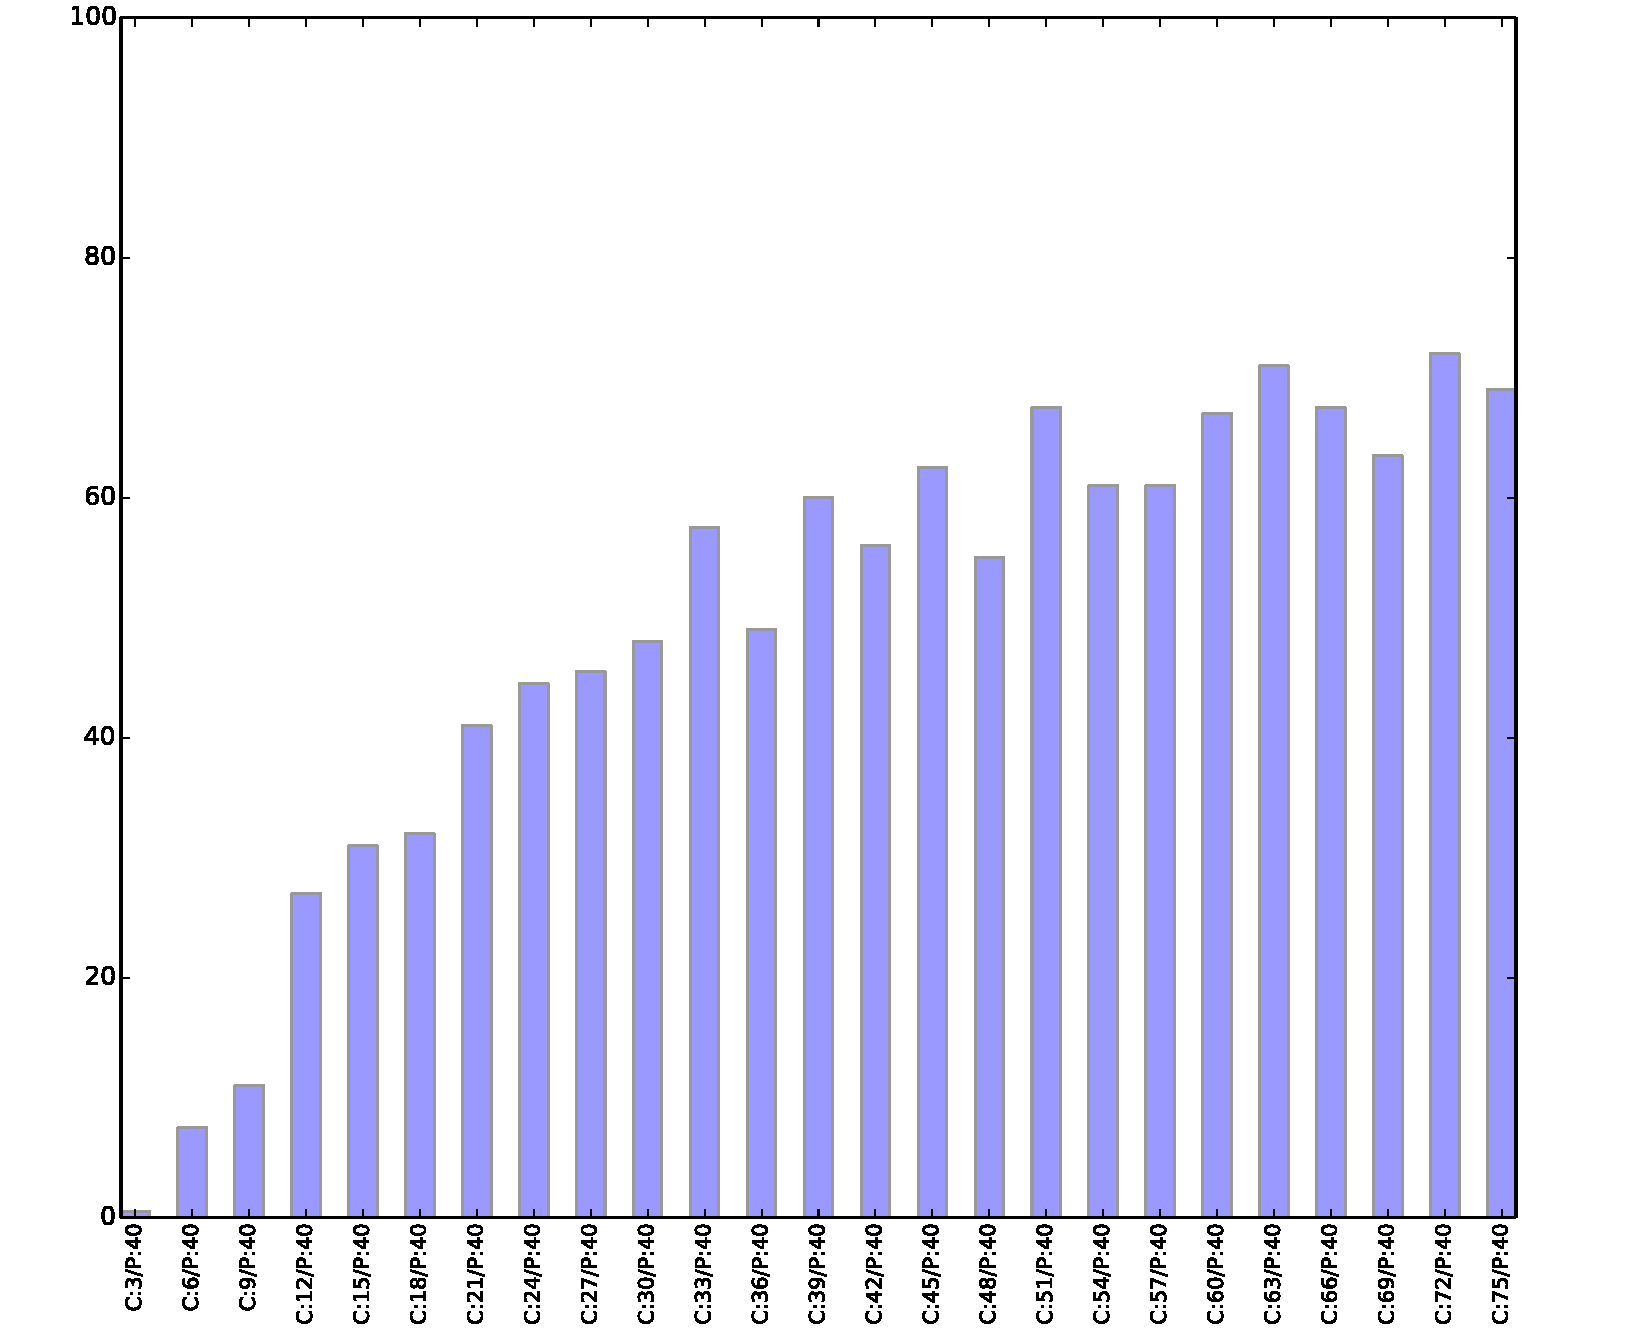
\includegraphics[width=0.78\textwidth]{images/C_G_CS_div5CS_solved.pdf}
  \caption[KG Algorithmus - Skalierung mit Anzahl Kandidaten]{KG Algorithmus - Skalierung mit Anzahl Kandidaten}
  \label{fig:c_g_cs_div5}
\end{figure}

Um zu messen wie der Algorithmus mit der Anzahl Lösungskandidaten skaliert, wurde eine Testreihe mit fixer Anzahl Probleme und variabler Anzahl Lösungskandidaten implementiert.

Die Eingabeparameter für die Abbildung \ref{fig:c_g_cs_div5} waren:
\begin{itemize}
	\item Grösse der Problemmenge: 40
	\item Anzahl der Lösungskandidaten: 3, 6, 9, 12, ..., 72, 75
\end{itemize}

Hier wurde bewusst eine zu kleine Problemmenge gewählt um nicht an die 100\% Marke zu kommen. Man sieht hier wiederum, dass sehr kleine Mengen ($3$, $6$, $9$ Kandidaten) praktisch gar nicht skalieren. Die Kurve steigt danach Steil an und flacht ab ca. 35 Lösungskandidaten ab, steigt jedoch weiter.